\section{Предрасчитанные данные}
\label{sec:Chapter2} \index{Chapter2}

Помимо очевидных оптимизаций, например изменения шага итерирования или уменьшения разрешения итогового изображения, для некоторых сцен возможны оптимизации, координально меняющие алгоритм рендеринга. Для рабочей сцены, т.е. для черный дыры, возможно одна из таких оптимизаций - можно использовать заранее расчитанные данные, чтобы не использовать метод Рунге-Кутты \eqref{eq:runge-kutte} множество раз в цикле, а просто взять необходимую информацию из этих предрасчитанных данных. Для черной дыры этими данными будут информация об итоговом угле отклонения $\phi$ луча на бесконечности для корректной отрисовки окружающей среды и информация о пересечении луча с аккреционного диска.

\subsection{Итоговый угол отклонения $\phi$ на бесконечности}
\label{subsec:precomputed_phi}

Начальный угол в разделе \ref{subsec:transition_from_decart_to_polar} приняли за ноль $\phi_{0} = 0$. Для итогового угла отклонения $\phi$ нельзя получить аналитическое выражение, однако можно заранее рассчитать итоговый угол $\phi$ при уходе луча на бесконечность и записать ее в качестве \textit{текстуры} (изображения), из которой затем будет выбираться необходимая информация. Текстуру удобно использовать, поскольку для текстур предлагается аппаратная линейная фильтрация на видеокарте между пикселями текстуры.

Итак, для рассчета итогового угла отклонения необходимо знать значения параметров $u$ и $\frac{du}{d\phi}$ из уравнения \eqref{eq:diffur}. Действительно, поскольку траектория света в окрестности черной дыры не зависит от вектора вращения, т.е. вектора плоскости, в которой луч совершает движение, то можно ограничиться только этими двумя параметрами. Таким образом, поскольку необходимо знать два параметра, то предрасчитанная текстура будет двумерной. Разумеется каждый пиксель будет хранить данные типа \textit{float32} (IEEE-754).

Рассчитать значения можно тем же методом Рунге-Кутты, но поскольку это предрассчет, то можно использовать более точные порядки и шаги итерирования.

В ходе итерирования луч также может попасть в горизонт событий и такой случай нужно как-то записать. В данной работе помимо итогового значения угла отклонения $\phi$ записывается еще маска, идентифицирующая попадание в черную дыру: если луч попал в черную дыру, то записывается значение $-1.0$, если луч ушел на бесконечность - записывается $1.0$. Таким образом каждому пикселю текстуры соответсвует набор из двух значений $\left(\phi, \text{mask}\right)$.

Осталось разобраться что будет означать ось абсцисс текстуры, а что будет означать ось ординат. Самое главное требование - компактность координат. Координаты должны пробегать все возможные значения, но при этом являться ограниченными. Примером неподходящего параметра является радиус $r$. Луч в алгоритме рендеринга черной дыры (см. раздел \ref{sec:Chapter1}) принимает следующие значения радиуса $r \in \left[r_{s}, +\infty\right]$ и этот параметр не подходит, поскольку может уйти на бесконечность. С другой стороны, параметр $u=\frac{1}{r} \in \left[0, \frac{1}{r_s}\right]$ вполне подходящий, т.к. область значений находится на конечном промежутке. Поэтому для оси абсцисс был выбран нормализованный обратный радиус:

\begin{equation}
\label{eq:sample_precompute_u}
    \frac{r_s}{r}=ur_s \in [0, 1].
\end{equation}

, a для оси ординат - угол:

\begin{equation}
\label{eq:sample_precompute_alpha}
    \left(\frac{\alpha}{\pi} + 0.5\right) \in \left[0, 1\right].
\end{equation}

, угол $\phi$ аналогичен углу с тем же названием из раздела \ref{subsec:transition_from_polar_to_decart} (см. рис. \ref{fig:transform_direction}). Напомню, что $\frac{du}{d\phi} = -\frac{1}{r} \cdot \tan{\phi}$.

Резюмируя, предрассчет будет выглядеть следующим образом: для каждого пикселя текстуры размером $(X, Y)$ с координатами $(x_i, y_i)$ будут линейно вычисляться обратный радиус и угол $phi$ по формулам, обратным формулам \eqref{eq:sample_precompute_u} и \eqref{eq:sample_precompute_alpha}:

\begin{equation}
\label{eq:precompute_u}
    u = \frac{1}{r} = \frac{1}{r_s} \cdot \frac{x_i}{X - 1}.
\end{equation}

\begin{equation}
\label{eq:precompute_alpha}
    \alpha = \pi\cdot\left(\frac{y_i}{Y - 1} - 0.5\right),
    \quad
    \frac{du}{d\phi} = -\frac{1}{r}\tan{\alpha}.
\end{equation}

, а зная $u$ и $\frac{du}{d\phi}$ уже по известному алгоритму можно рассчитать итоговый угол отклонения $\phi$ (см. рис. \ref{fig:precomputed_phi}).

\begin{figure}[h]
    \centering
    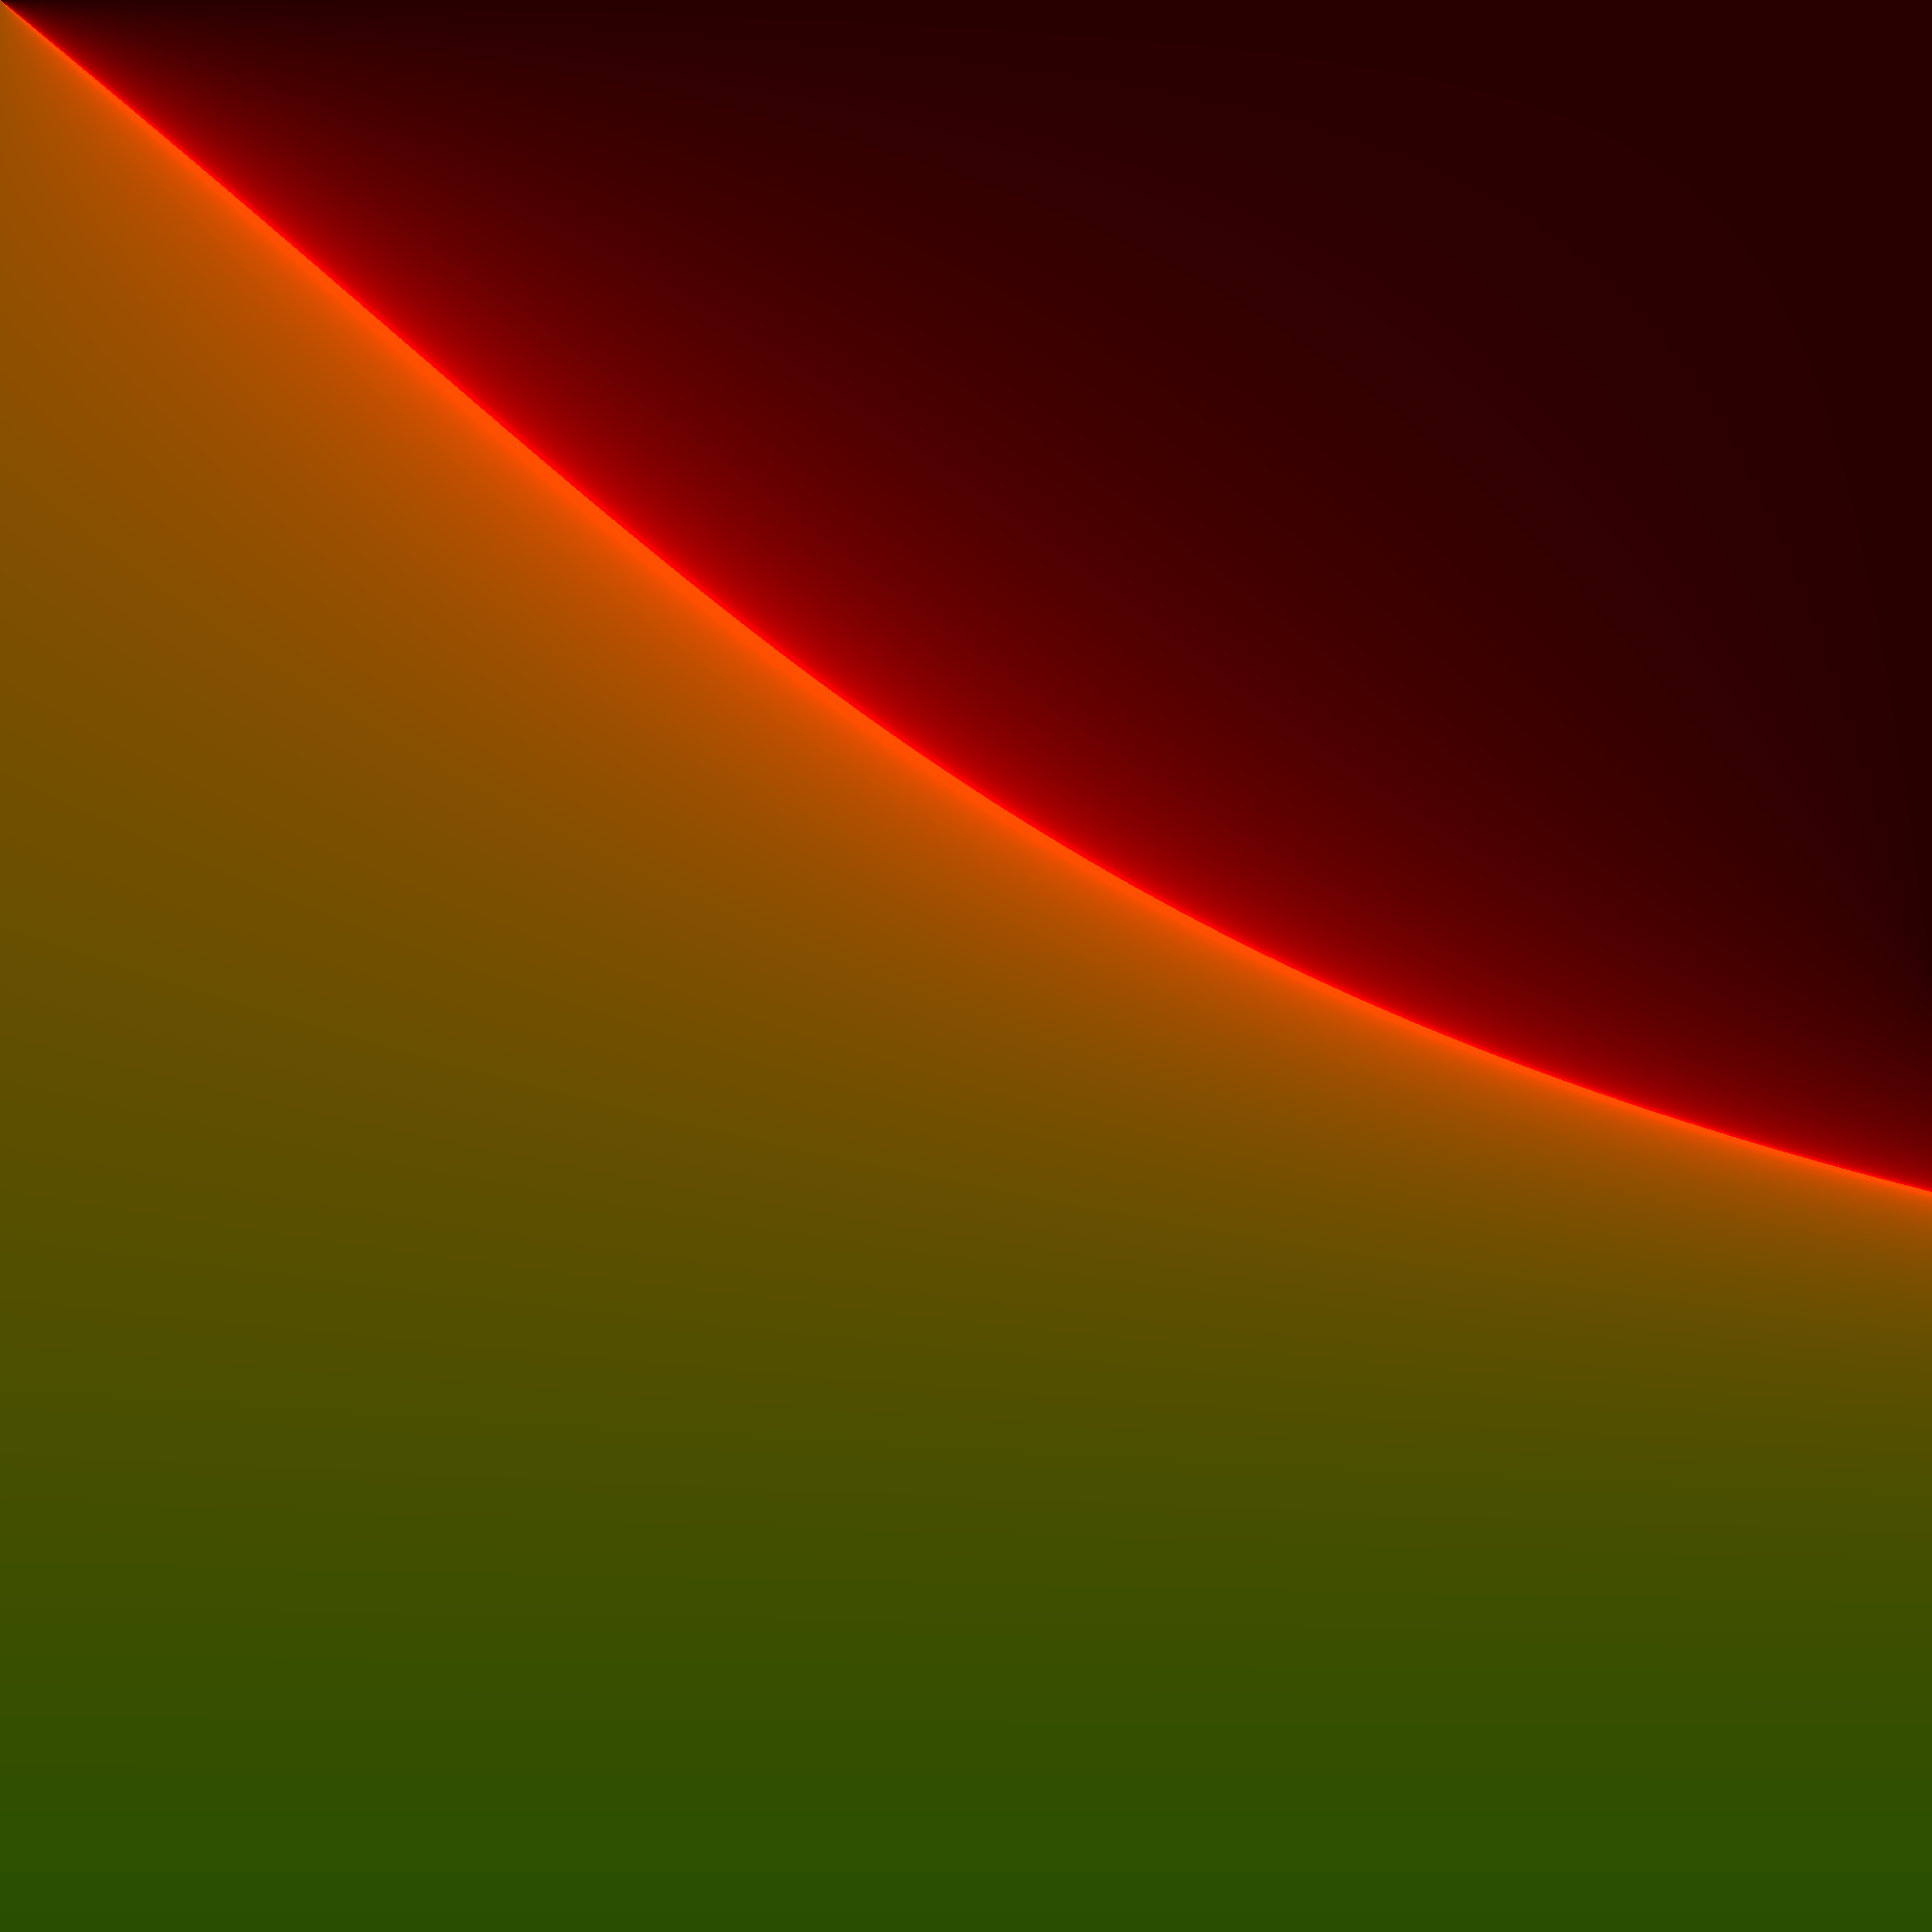
\includegraphics[width=0.8\linewidth]{PrecomputedPhi}
    \caption{Предрасчитанная текстура размером $(2000, 2000)$. Красный канал отвечает за итоговый угол отклонения $\phi$, а зеленый канал - за маску, идентефицирующую попадание в горизонт событий.}
    \label{fig:precomputed_phi}
\end{figure}

\newpage

\subsection{Пересечение луча с аккреционным диском}

\begin{figure}[h]
    \centering
    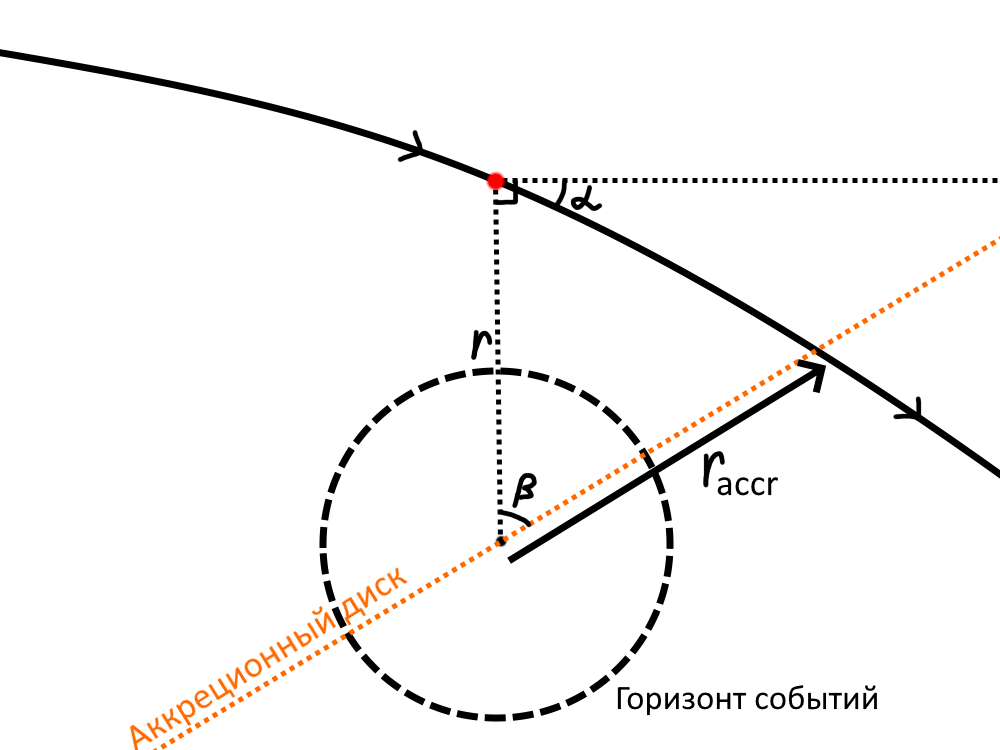
\includegraphics[width=0.8\linewidth]{Angles-Overview}
    \caption{Схема параметров для предрассчета радиуса пересечения $r_{accr}$ аккреционного диска. Сплошной кривой указана траектория света вблизи черной дыры, оранжевым пунктиром - линия пересечения плоскости аккреционного диска и плоскости движения луча света.}
    \label{fig:angle_overview}
\end{figure}

В случае аккреционного диска, зависимость плотности которого радиальна, согласно разделу \ref{subsec:accr_disk}, достаточно лишь знать радиус пересечения с аккреционным диском $r_{accr}$, при условии, что диск является очень тонким.

Для того, чтобы узнать радиус пересечения с аккреционным диском $r_{accr}$ нужно дополнительно знать угол $\beta$ до пересечения с аккреционными диском в плоскости движения луча света, помимо параметров $u$ и $\alpha$ из прошлого раздела \ref{subsec:precomputed_phi} (см. рис. \ref{fig:angle_overview}). Поскольку необходимо знать три параметра для нахождения искомого $r_{accr}$, то текстура будет трехмерной размером $(X, Y, Z)$.

Ось абсцисс и ось ординат текстуры такие же, как в прошлом разделе \ref{subsec:precomputed_phi}. А вот ось аппликат будет с координатами равными:

\begin{equation}
\label{eq:sample_precompute_beta}
    \frac{\beta}{\pi} \in \left[0, 1\right].
\end{equation}

Таким образом, алгоритм вычисления радиуса пересечения с аккреционным диском $r_{accr}$ следующий: для каждого пикселя в предрассчитанной текстуре с координатами $(x_i, y_i, z_i)$ вычисляются $u$ и $\alpha$ по формулам \eqref{eq:precompute_u} и \eqref{eq:precompute_alpha}, а параметр $\beta$ вычисляется по формуле, обратной \eqref{eq:sample_precompute_beta}:

\begin{equation}
\label{eq:precompute_beta}
    \beta = \pi \cdot \frac{z_i}{Z - 1}.
\end{equation}

Зная $u$, $\frac{du}{d\phi}$ и $\beta$ легко вычислить искомое значение $r_{accr}$. Для этого используем все тот же метод Рунге-Кутты, однако заменяем всего пару вещей: начальное значение $\phi=\phi_0$ делаем равным $\beta$ и добавляем условие на пересечение с аккреционным диском, а именно при достижении параметра $\phi$ значения $\pi$ или больше, считаем пересечения луча света с аккреционным диском произошедшим и записываем радиус $r = \frac{1}{u}$ в пиксель. Если луч ушел на бесконечность, то нужно записать какой-то идентифицирующее это значение, например большое число. Если же луч попал в горизонт событий, то нужно использовать еще одно специальное значение, например ноль.

Обычно при наблюдении черной дыры хорошо видно два аккреционных диска, возникающих при первом и втором пересечениях траектории света с аккреционным диском, поэтому разумно в текстуре сохранять набор из двух значений: радиусы первого и второго пересечений с аккреционным диском $r_{accr1}$ и $r_{accr2}$.

Рисунки \ref{fig:precomputed_accr_beta_1pi4} и \ref{fig:precomputed_accr_beta_3pi4} показывают предрасчитанные радиусы $r_{accr}$ для первого и второго пересечений с аккреционным диском для значений $\beta = \frac{1\pi}{4}$ и $\beta = \frac{3\pi}{4}$ соответственно. Наблюдаются три зоны: черная - либо траектория света ушла в горизонт событий, не успев пересечься с аккреционным диском, либо первый пересечение произошло, а второе - нет, либо первое и второе пересечения с аккреционным диском произошли; зеленая - траектория света пересекла плоскость аккреционного диска лишь один раз; желтая - траектория света не пересекла ни разу плоскость аккреционного диска.

\newpage

\begin{figure}
    \centering
    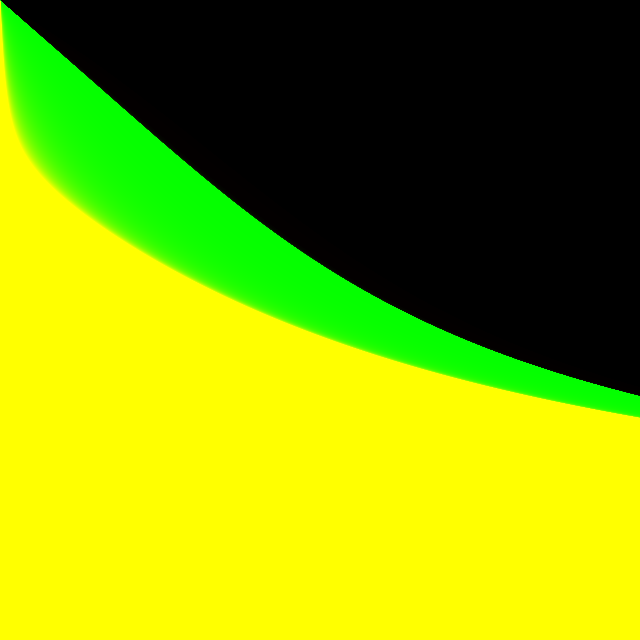
\includegraphics[width=0.45\linewidth]{PrecomputedAccrBetapi4}
    \caption{Предрасчитанная текстура размером $(640, 640, 128)$, но выбрано значение $\beta = \frac{\pi}{4}$. Красный канал отвечает за радиус первого пересечения с аккреционным диском $r_{accr1}$, а зеленый канал - за радиус первого пересечения с аккреционным диском $r_{accr2}$.}
    \label{fig:precomputed_accr_beta_1pi4}
\end{figure}

\begin{figure}[h]
    \centering
    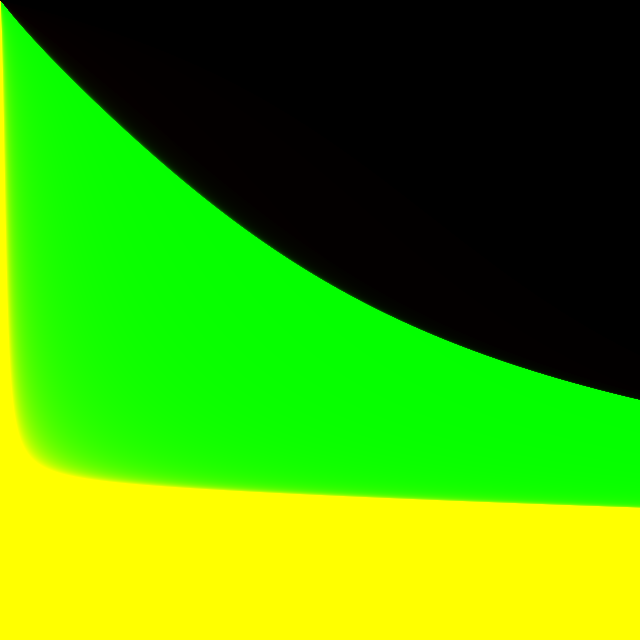
\includegraphics[width=0.45\linewidth]{PrecomputedAccrBeta3pi4}
    \caption{Предрасчитанная текстура размером $(640, 640, 128)$, но выбрано значение $\beta = \frac{3\pi}{4}$. Красный канал отвечает за радиус первого пересечения с аккреционным диском $r_{accr1}$, а зеленый канал - за радиус первого пересечения с аккреционным диском $r_{accr2}$.}
    \label{fig:precomputed_accr_beta_3pi4}
\end{figure}

\newpage

\subsection{Использование предрасчитанных данных для рендеринга черной дыры}
\label{subsec:precompute_black_hole_rendering}

Как было сказано выше, теперь для рендеринга черной дыры необходимо только использовать предрасчитанные данные и затем обработать их.

Для аккреционного диска, выбирая данные по координатам \eqref{eq:sample_precompute_u}, \eqref{eq:sample_precompute_alpha} и \eqref{eq:sample_precompute_beta}, можно получить данные о радиусе пересечений с аккреционным диском, а зная их, можно легко определить цвет в месте пересечения (как я и говорил выше, цвет диска имеет исключительно радиальную зависимость в данной работе).

Для итогового угла отклонения $\phi$ можно рассчитать как измениться позиция луча света $\mathbf{a}$ на бесконечности, а поскольку это происходит на бесконечности, то в пределе можно сказать, что позиция $\mathbf{a}$ и направление $\mathbf{d}$ луча света будут сонаправлены, а значит легко можно будет взять цвет из окружающей среды (см. раздел \ref{subsubsec:goes_to_infinity}).

Единственным минусом предрасчитанных данных является допущение малой толщины аккреционного диска.

\begin{figure}[h]
    \centering
    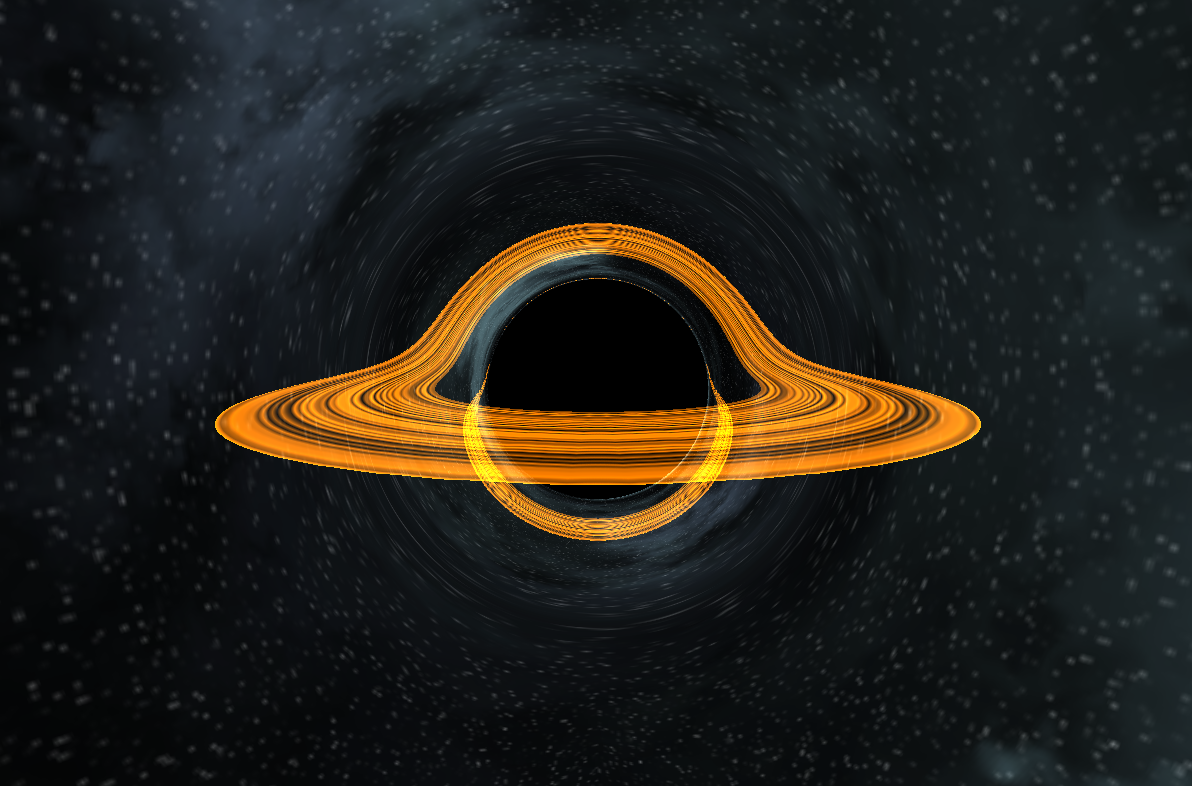
\includegraphics[width=1.0\linewidth]{BlackHolePrecomputed}
    \caption{Рендеринг черной дыры с использованием предрасчитанных данных.}
    \label{fig:black_hole_precomputed}
\end{figure}

\newpage